\documentclass{beamer}
\usepackage{graphicx} % For including images (e.g., QR code)
\usepackage{hyperref} % For creating hyperlinks
\usepackage{xcolor}   % For color customization
%\usepackage{fontspec} % Uncomment if using LuaLaTeX or XeLaTeX for font support

% -----------------------------------------------------------------------------
% Hyperlink Colors Configuration
% -----------------------------------------------------------------------------
\hypersetup{
    colorlinks=true,   % Enable colored links instead of boxed links
    linkcolor=blue,    % Internal link color
    urlcolor=cyan      % External link (URL) color
}

% -----------------------------------------------------------------------------
% Custom Footer Configuration
% -----------------------------------------------------------------------------
\setbeamertemplate{footline}{%
  \leavevmode%
  \hbox{
    \begin{beamercolorbox}[wd=.33\paperwidth,ht=2.25ex,dp=1ex,leftskip=.3cm]{author in head/foot}%
      Wireless Club at Northeastern University%
    \end{beamercolorbox}%
    \begin{beamercolorbox}[wd=.33\paperwidth,ht=2.25ex,dp=1ex,center]{author in head/foot}%
      Yagi Antenna Workshop%
    \end{beamercolorbox}%
    \begin{beamercolorbox}[wd=.33\paperwidth,ht=2.25ex,dp=1ex,rightskip=.3cm plus1fil]{author in head/foot}%
      \insertframenumber/\inserttotalframenumber \hspace{1em} Fall 2024%
    \end{beamercolorbox}}%
  \vskip0pt%
}

%  Slide: Title Information
\title{Yagi Antenna Workshop}
\subtitle{Building a Tape Measure Antenna}
\author{Northeastern University Wireless Club - W1KBN}
\date{September 9, 2024}

\begin{document}

% Slide: Title with QR Code for Sign-In
\begin{frame}
    \titlepage
    \vspace{-1cm} % Adjust overall vertical positioning of content
    \begin{center}
        \textbf{Sign in here!} \\
        
\includegraphics[width=0.30\textwidth]{qrcode.png} % QR code image
        \vspace{-0.3cm} % Adjust space between text and QR code
        \\
        {\small \url{https://l.w1kbn.org/signin}} % Sign-in URL under QR code
    \end{center}
\end{frame}

% Slide: Welcome
\begin{frame}
    \frametitle{Welcome to Our First Workshop!}
    \begin{itemize}
        \item Welcome to the Wireless Club's first workshop of the semester!
        \item Who we are:
        \begin{itemize}
            \item We are Northeastern University's Wireless Club, a student group passionate about electronics, antennas, and wireless technologies.
            \item Our workshops are designed to be accessible for all skill levels—whether you have experience or not, you’re in the right place.
        \end{itemize}
        \item Today’s Plan:
        \begin{itemize}
            \item Introduction to HAM Radio and Antennas
            \item Step-by-step Yagi Antenna build using a tape measure and basic materials
            \item Q&A and hands-on assembly
        \end{itemize}
        \item Visit our website for more: \url{https://nuwireless.org/}
    \end{itemize}
\end{frame}

% Slide: Welcome and Sign-In Information
\begin{frame}
    \frametitle{Welcome!}
    \begin{itemize}
        \item Wireless Club Meetings: 7 PM Thursdays @ 503 Hayden (Free Pizza!)
        \item Workshop Meetings: 7 PM Mondays @ East Village, Room 010
        \item Join our Slack: \url{https://neuwireless.slack.com/join/signup}
        \item Join our mailing list: \url{http://eepurl.com/gduCIr}
        \item Scope of today's workshop:
        \begin{itemize}
            \item Rapid-Fire Ham Radio Overview
            \item Antennas 101
            \item The Build: \url{https://www.instructables.com/The-Tape-Measure-Antenna/}
        \end{itemize}
        \item Sign-in: \url{https://l.w1kbn.org/signin}
    \end{itemize}
\end{frame}

% Slide: Common Terms and Abbreviations
\begin{frame}
    \frametitle{Common Terms and Abbreviations}
    \begin{itemize}
        \item \textbf{HAM Radio} – Amateur Radio, used for personal, non-commercial communication.
        \item \textbf{VHF} – Very High Frequency (radio waves in the 30 MHz to 300 MHz range).
        \item \textbf{SWR} – Standing Wave Ratio, a measure of the efficiency of the antenna's power transfer.
        \item \textbf{RG-58 Cable} – A type of coaxial cable used for radio frequency signals.
        \item \textbf{BNC Connector} – A common radio-frequency connector used for coaxial cable.
        \item \textbf{Impedance Matching} – Adjusting the antenna so the electrical load matches the transmission line for better power transfer.
    \end{itemize}
\end{frame}

% Slide: Explanation of HAM Radio
\begin{frame}
    \frametitle{What is HAM Radio?}
    \begin{itemize}
        \item A hobby and service that allows individuals to communicate using designated radio frequencies for personal, non-commercial purposes.
        \item HAM radio operators can use equipment like handheld transceivers (walkie-talkies) to communicate.
        \item Different modes include voice (talking), Morse code (using beeps), and data (sending text over the airwaves).
    \end{itemize}
\end{frame}

% Slide: Yagi Antenna Overview
\begin{frame}
    \frametitle{Yagi Antenna Overview}
    \begin{itemize}
        \item A \textbf{Yagi antenna} is a type of directional antenna, which means it focuses the radio signal in a specific direction.
        \item It consists of:
        \begin{itemize}
            \item \textbf{Driven Element} – The part that connects to the transmitter/receiver (this part sends or receives the signal).
            \item \textbf{Reflector} – A passive element that bounces signals back towards the driven element to strengthen them.
            \item \textbf{Director(s)} – Elements that help further focus the signal in one direction.
        \end{itemize}
        \item Yagi antennas are commonly used in amateur radio, TV reception, and Wi-Fi because they are great for long-distance communication.
    \end{itemize}
\end{frame}

% Slide: Bill of Materials slide with two columns (Materials on the left, Tools on the right)
\begin{frame}
    \frametitle{Bill of Materials}
    \scriptsize % Use smaller text size to fit content
    
    \begin{columns}
        % Left column: Materials Needed
        \begin{column}{0.5\textwidth}
            \textbf{Materials Needed:}
            \begin{itemize}
                \item \textbf{PVC Pipe (3/4” Schedule 40)} – Minimum 25 inches
                \item \textbf{Hose Clamps} – 6 clamps, large enough to fit around the PVC pipe
                \item \textbf{PVC Tee} – 1 piece (3/4”)
                \item \textbf{PVC Crosses} – 2 pieces (3/4”)
                \item \textbf{RG-58 Cable} – 8 feet long, with a connector on one end (e.g., female BNC)
                \item \textbf{Wire} – 5 inches of wire (e.g., 18 gauge solid copper wire or similar)
                \item \textbf{Rosin Core Solder} – For soldering connections
                \item \textbf{Tape Measure} – 1 inch wide
                \item \textbf{PVC Glue} – For securing PVC joints
            \end{itemize}
        \end{column}
        
        % Right column: Tools Needed
        \begin{column}{0.5\textwidth}
            \textbf{Tools Needed:}
            \begin{itemize}
                \item \textbf{Soldering Iron} – For soldering wire connections
                \item \textbf{Tape Measure} – For measuring lengths accurately
                \item \textbf{Pipe Cutters} – To cut the PVC pipe
                \item \textbf{Wire Stripper} – For stripping insulation off wires
                \item \textbf{Shears or Scissors} – To cut the tape measure
                \item \textbf{Sandpaper} – To smooth cut edges of metal parts
                \item \textbf{SWR Meter} – For testing antenna performance
                \item \textbf{Screwdriver/Wrench} – To tighten hose clamps
            \end{itemize}
        \end{column}
    \end{columns}
\end{frame}


% -----------------------------------------------------------------------------
% Step-by-Step Slides (Cutting, Installing, Soldering, Adjusting Antenna)
% -----------------------------------------------------------------------------
% Step 1: Cutting the Elements
\begin{frame}
    \frametitle{Step 1: Cutting the Elements}
    \begin{itemize}
        \item Cut two PVC pieces (17.5" and 7") for the frame.
        \item Disassemble the tape measure and cut three elements:
        \begin{itemize}
            \item Director: 35 1/8"
            \item Driven Elements: Two 17 3/4"
            \item Reflector: 41 3/8"
        \end{itemize}
        \item Sand the ends of the elements for safety and soldering.
    \end{itemize}
    \begin{center}
    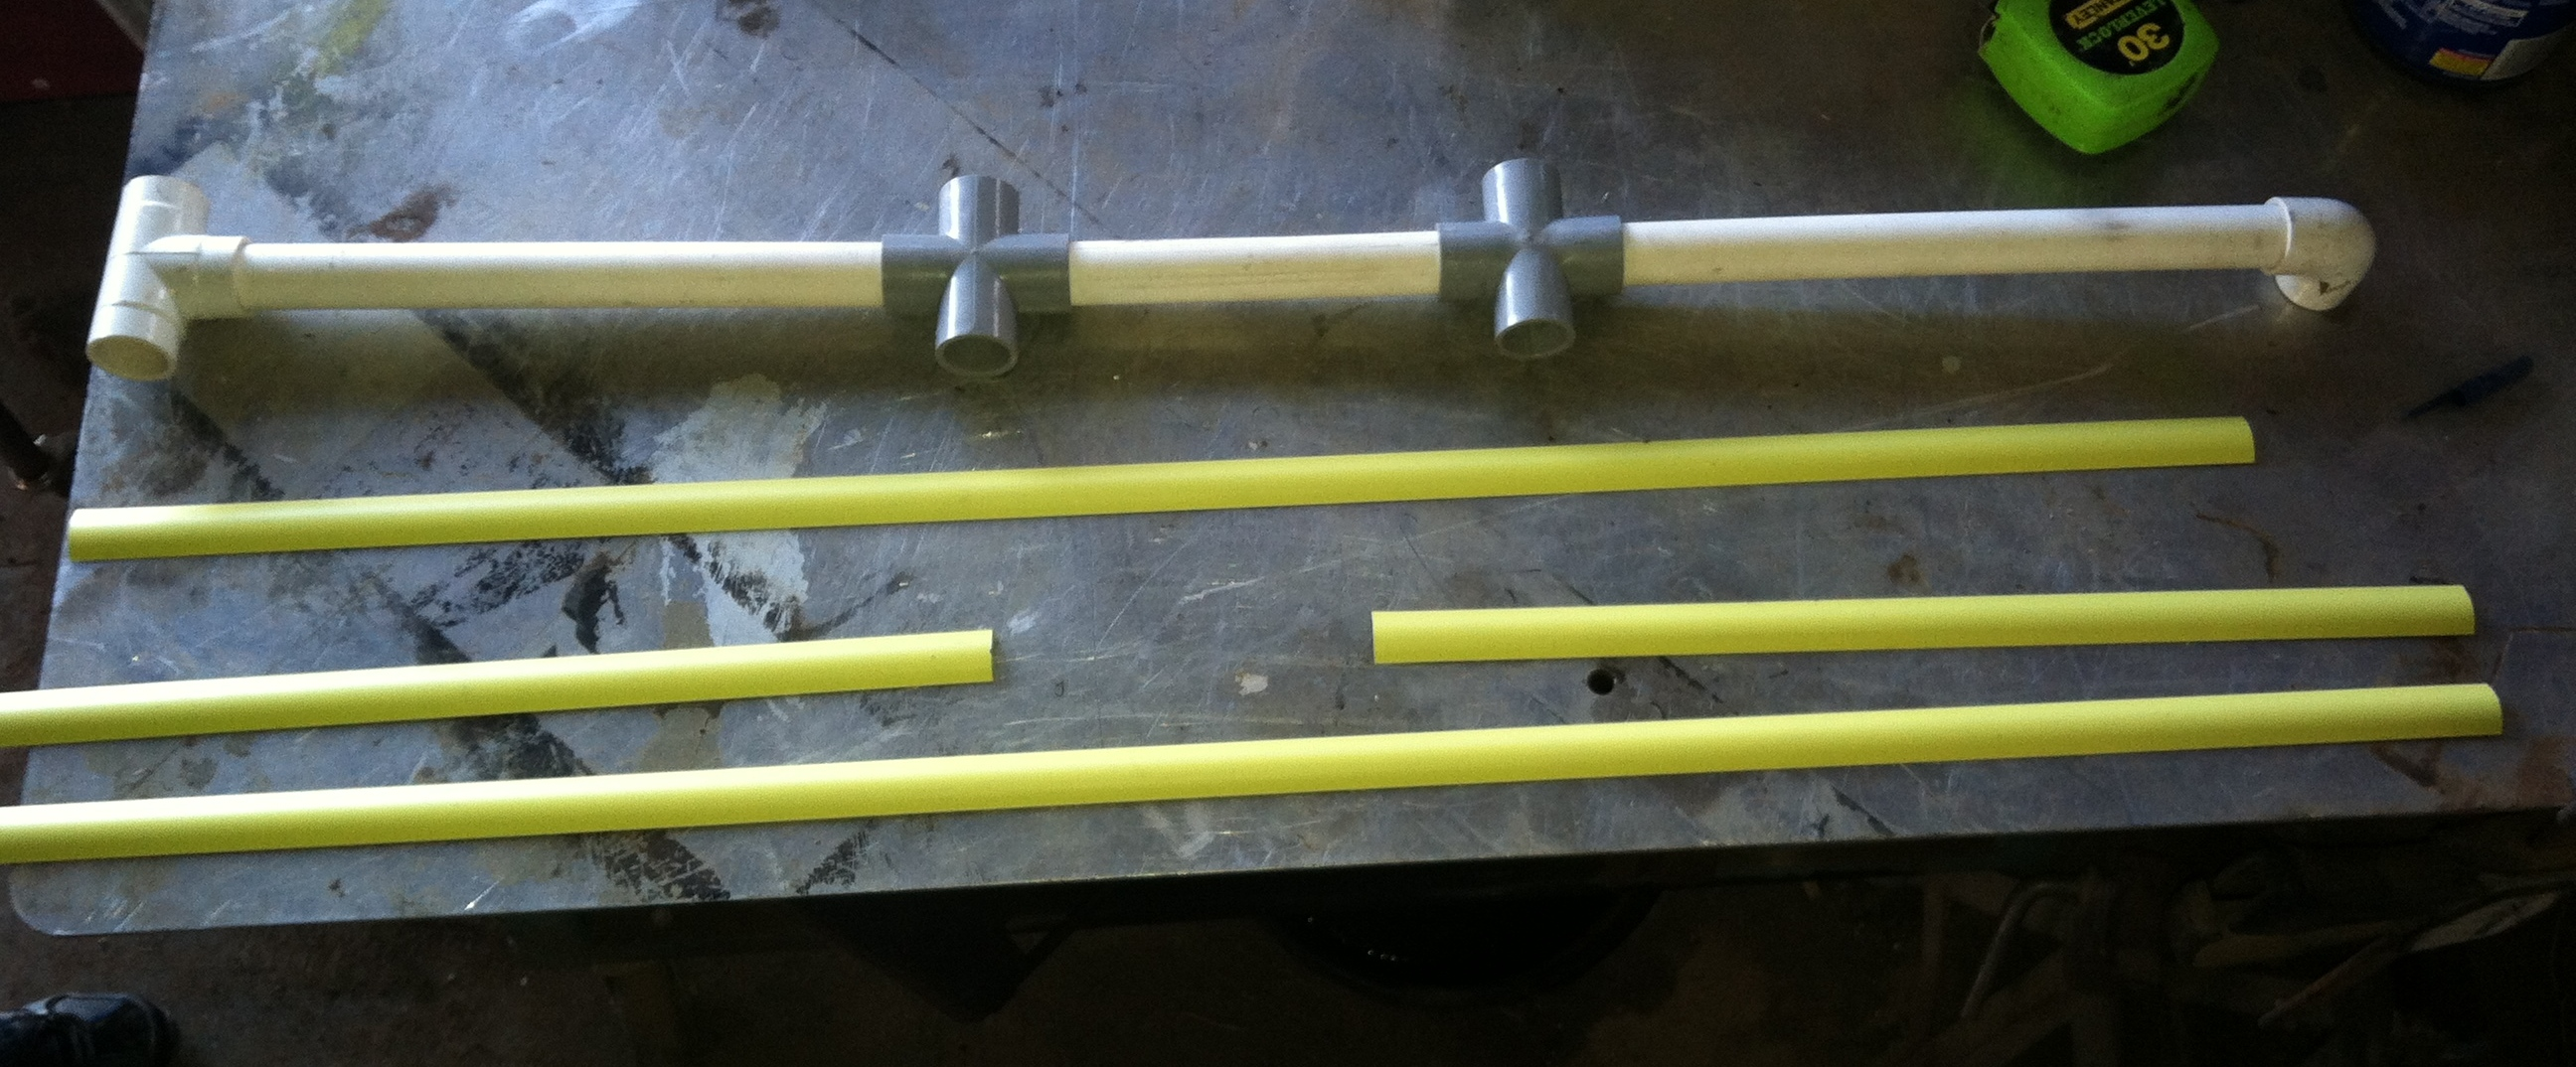
\includegraphics[width=0.7\textwidth]{cutting_elements.jpg} % Replace with appropriate image
    \end{center}
\end{frame}

% Step 2: Installing the Elements
\begin{frame}
    \frametitle{Step 2: Installing the Elements}
    \begin{itemize}
        \item Attach the Director element at the front with hose clamps.
        \item Install the driven elements and ensure they are spaced 1" apart.
        \item Secure the Reflector element at the rear of the antenna.
    \end{itemize}
%    \includegraphics[width=0.5\textwidth]{installing_elements.jpg} % Replace with appropriate image
\end{frame}

% Step 3: Soldering the Wires
\begin{frame}
    \frametitle{Step 3: Soldering the Wires}
    \begin{itemize}
        \item Tin the ends of the driven elements with solder.
        \item Solder the RG-58 cable: Inner wire to one driven element, outer to the other.
        \item Use a 5" wire to connect the two driven elements.
    \end{itemize}
    \begin{center}
        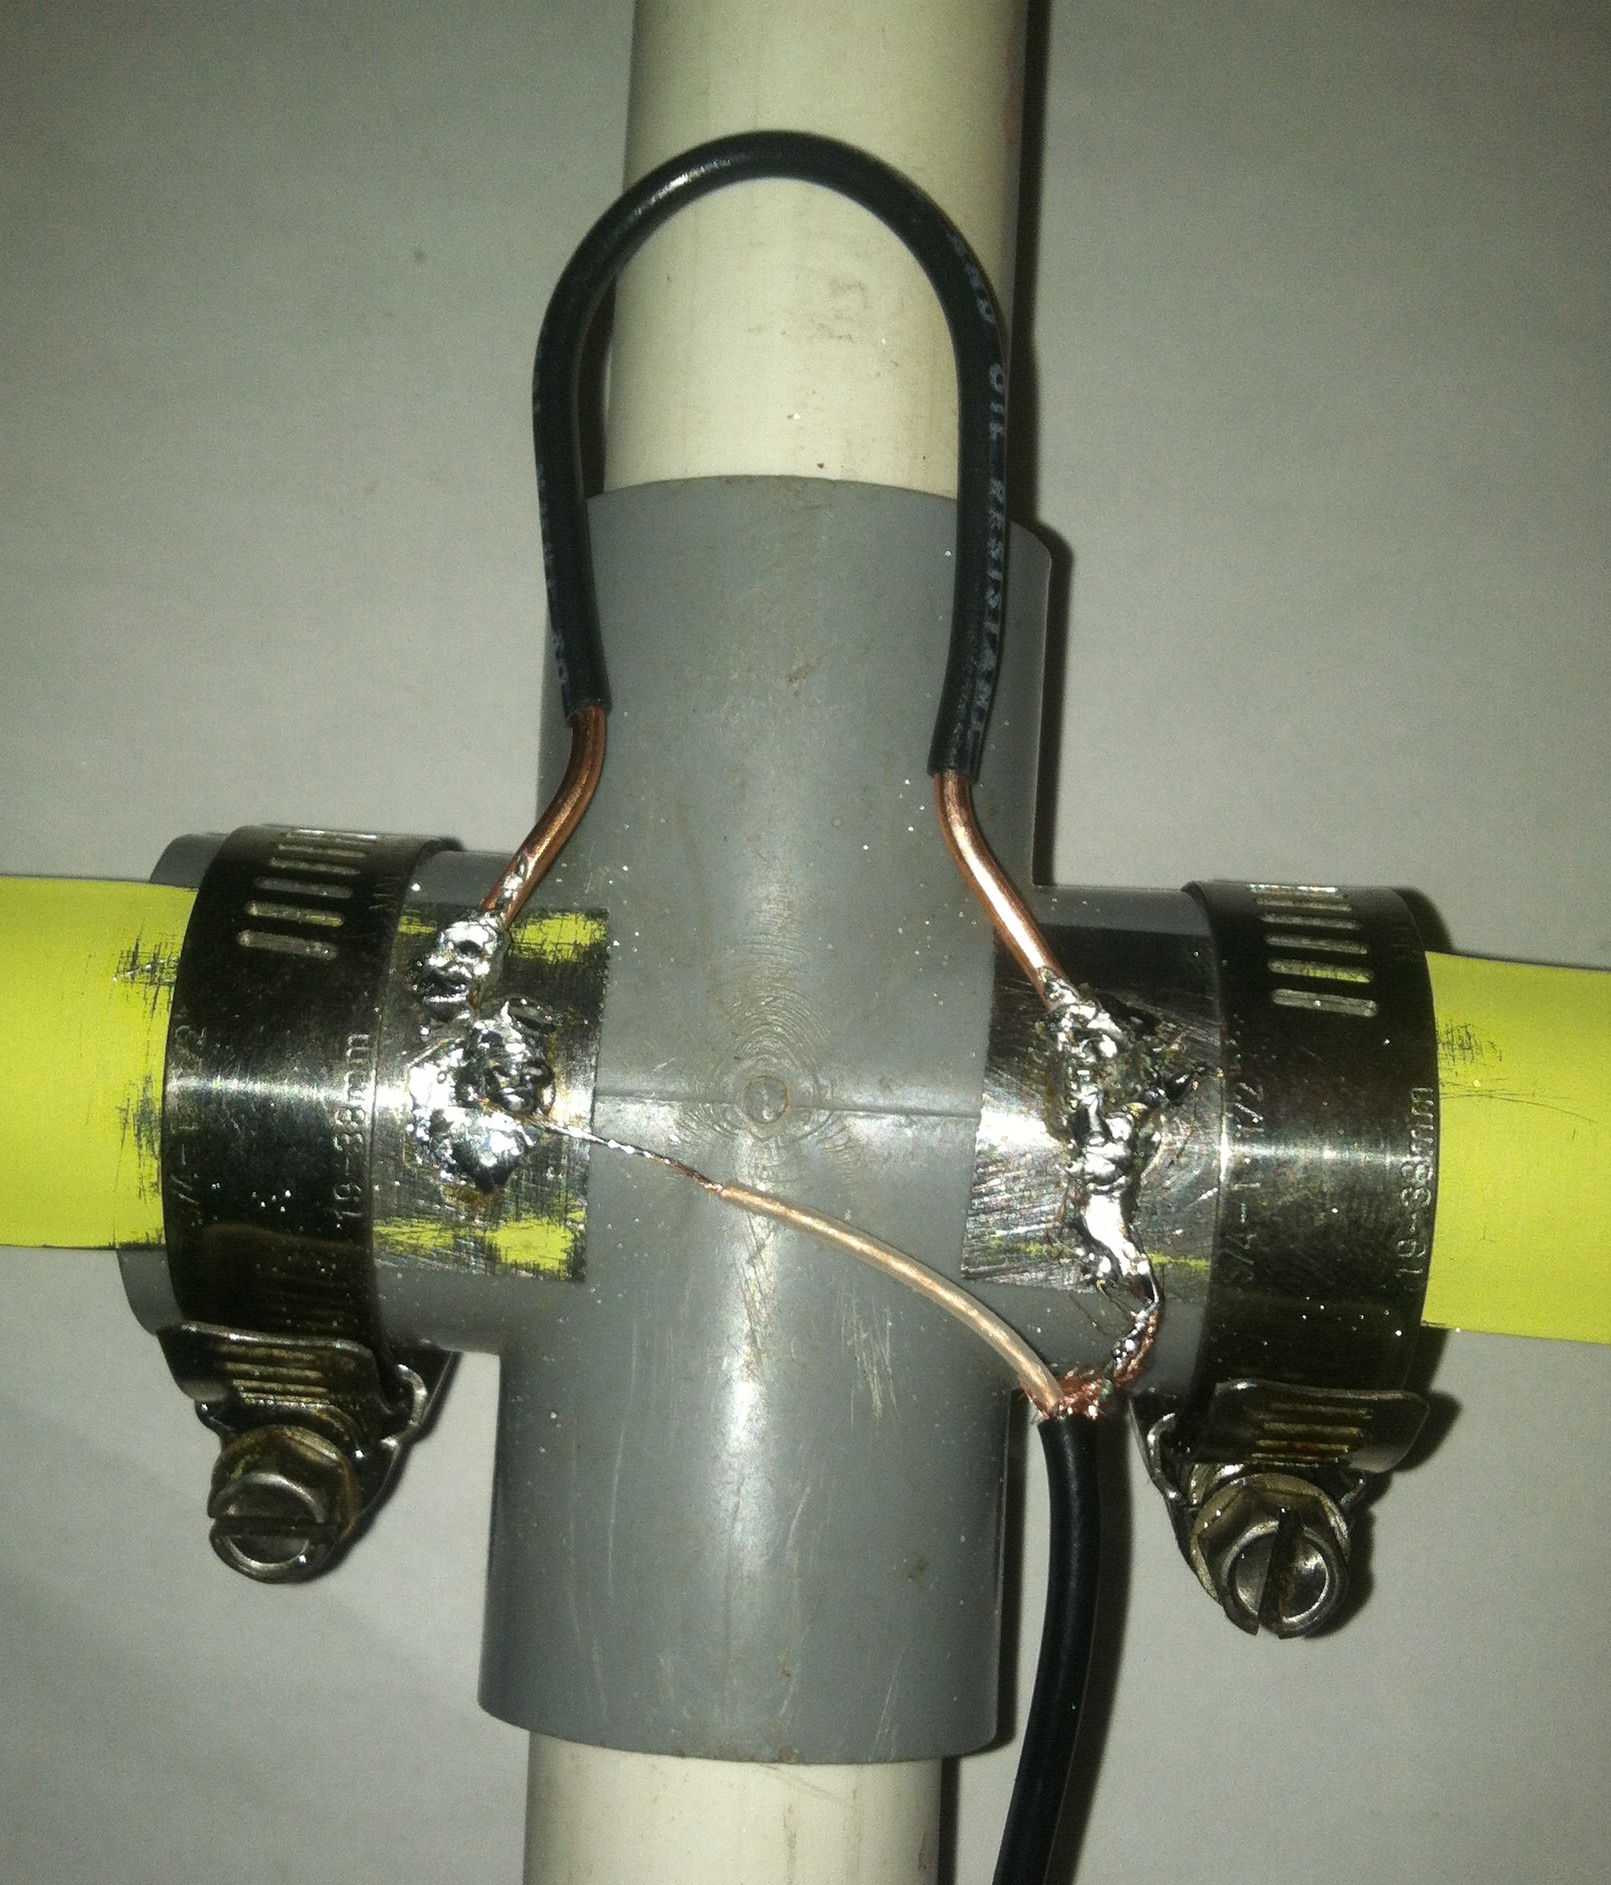
\includegraphics[width=0.4\textwidth]{soldering-1.jpg}
        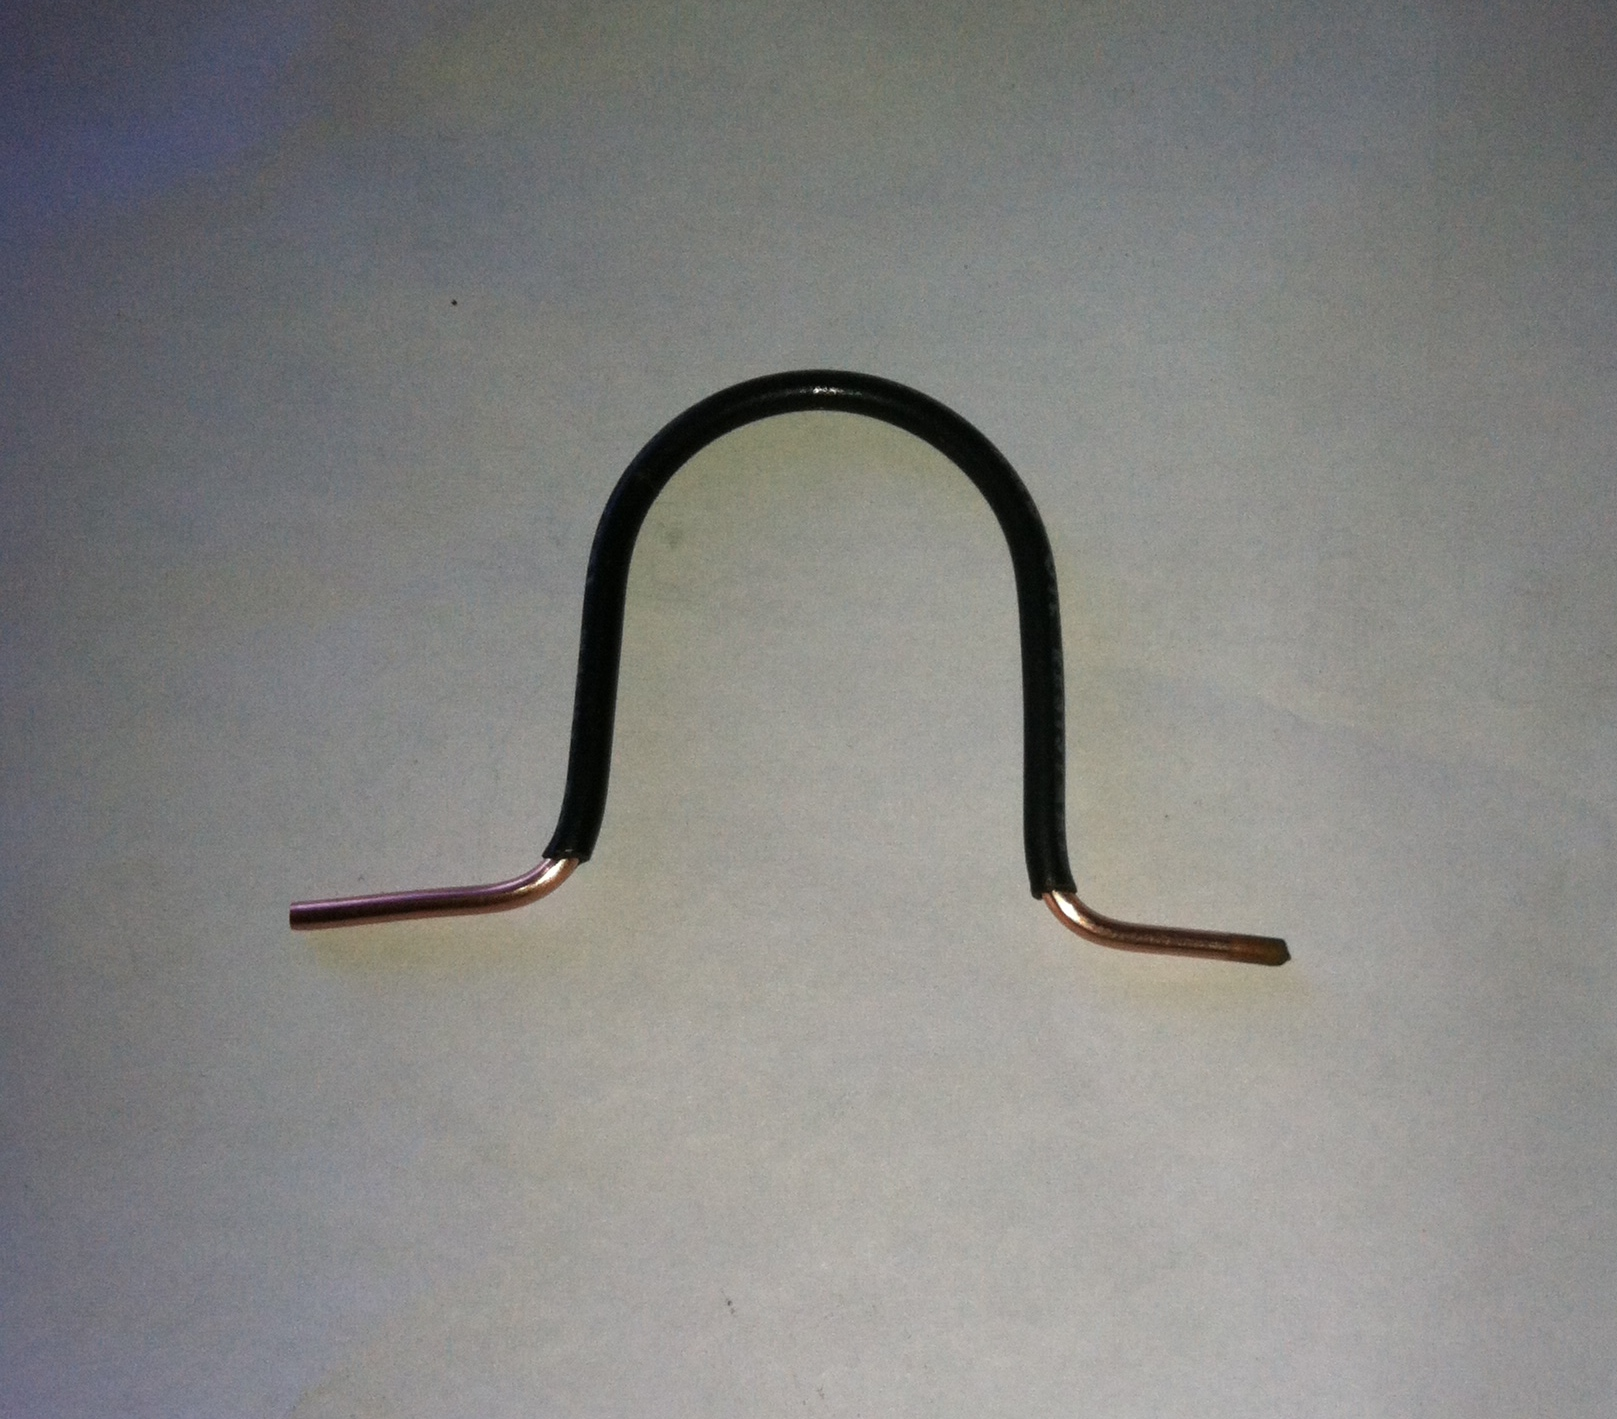
\includegraphics[width=0.4\textwidth]{soldering-2.jpg}
    \end{center}
\end{frame}

% Step 4: Adjusting the Antenna
\begin{frame}
    \frametitle{Antenna Adjustment} 
    \begin{itemize}
        \item Use an SWR meter to tune the antenna. 
        \item Adjust driven elements if SWR reading exceeds 1.2:1. 
        \item Ensure radio is off when adjusting. 
    \end{itemize} 
   % \includegraphics[width=0.4\textwidth]{adjusting_antenna.jpg}
\end{frame}

% Slide: Contact Us
\begin{frame}
    \frametitle{Contact Us}
    \begin{itemize}
        \item If you have any questions or want to learn more, feel free to reach out!
        \item Workshop Team Emails: \\
        \{\href{mailto:elarbi.m@northeastern.edu}{elarbi.m}, 
        \href{mailto:aviedov.v@northeastern.edu}{aviedov.v}, 
        \href{mailto:meaney.ma@northeastern.edu}{meaney.ma}\}[at]northeastern[d0t]edu
        \item General Workshop Email: \href{mailto:workshops@nuwireless.org}{workshops}[at]nuwireless[d0t]org
        \item Website: \url{https://nuwireless.org/}
        \item Visit us at: Hayden Hall, Room 503
    \end{itemize}
    \vspace{1cm}
    \begin{flushright}
        \footnotesize{© 2024 Northeastern Wireless Club} \\
        \footnotesize{Design: \href{https://melarbi.com}{Muhammad Elarbi}, based on LaTeX Beamer}
    \end{flushright}
\end{frame}

% Slide: References
\section{References} 
\begin{frame} 
    \frametitle{References} 
    \begin{itemize} 
        \item Original design by Joe Leggio, WB2HOL (\url{http://theleggios.net/wb2hol/projects/rdf/tape_bm.htm}) 
        \item Additional designs: KC0TKS (\url{http://www.kc0tks.org}) and NT1K (\url{http://nt1k.com}) 
        \item This workshop presentation is based on the project tutorial by jcoman (\url{https://www.instructables.com/The-Tape-Measure-Antenna/}).
        \item All images used in this presentation are sourced from jcoman's tutorial on Instructables.
    \end{itemize}
\end{frame}
\end{document}